\section{Kerekek Pid Szabalyzo hangolas}

A pid, a legelterjedtebb szabályozó egyszerű feladatok elvégzésére, esetünkben is elegendő a kerekek szögsebesség szabályzására kerekenkénti egy PID szabályzóval. A PID szoftveresen fut a uBlaze processzoron. Bemenete egy előírt forgási sebesség \degree/s -ban és kimenete egy -32000 és 32000 egész típusú értek. A kimenti érteke a PWM kitöltési tényezőt jeleni, az előjel pedig a beavatkozás irányát.
Matlab/Simulink környezetben használva a Robotix Toolbox segítségével direktben pwm beavatkozó referencia érteket írtam elő a motoroknak. A beavatkozó jel előállítása és elküldési a fizikai eszköznek 0-100\%-ig 10\% lépcsőkben, amelyek 0\% kitöltésekkel vannak megszakítva. A mért adatokat rosbag csomagba mentve majd a System Identification Toolbox használatával identifikáljuk a rendszer modellt. A rendszer bemenete egy beavatkozó jel, ami fizikailag feszültségnek fele meg 0V és 12V között. A kimenetek a forgási sebesség.
A mert adatokat Matlab/System Identification használatával megbecsüljük a rendszer modelleket. Nemlinearis modellt becslünk 
Hammerstein-Wiener model \cite{matlabhwmmodel} használva, 1 kimenet és 1 bemenet, a lineáris átviteli függvény fokszáma:
zerusok nb = 2, pólusok nf = 3, késés a bemenet és a kimenet között nk = 1. A becsült adatok 94\%-ban megfelelnek a mert rendszernek.          

A méréseket a robot kerekei és a talaj érintkezése nélkül végeztem.
A becsült modellt a bemenet 50/\%  körül linearizáljuk és a linearizált modellből átviteli függvényt készítünk. 
$tf = tf(linearize(model,16000));$ utasítást használva Matlab környezetben. A linearizált modellt Matlab/PidTuning eszközt használva behangolunk, kiszámítjuk a megfelelő PID szabályzó paramétereit.


\tikzstyle{block} = [draw, fill=white, rectangle, 
    minimum height=3em, minimum width=6em]
\tikzstyle{sum} = [draw, fill=white, circle, node distance=1cm]
\tikzstyle{matlab} = [draw, fill=white, circle, node distance=1cm]
\tikzstyle{input} = [coordinate]
\tikzstyle{output} = [coordinate]
\tikzstyle{pinstyle} = [pin edge={to-,thin,black}]
\begin{center}
\begin{tikzpicture}[auto, node distance=2cm,>=latex']

   \node [block] (matlab) {Matlab/Simulink};
   \node [block, right of=matlab, node distance=4cm] (system) {System};
   \node [block, below of=system] (rosbag) {ROS bag};

    \node [right of=matlab,fill=black,inner sep=1.2pt,node distance=62] (umid) {};
    \draw [->] (matlab) -- (system);
%---------------- 
    \path (system.north east)--(system.south east) foreach \j in {1,...,2} {%
        coordinate [pos=1/3*\j] (z\j)
    };
    
    \foreach \i/\name/\nameNode/\text  in {1/{Omega}/{Om}/{$    \Omega$},2/{Current}/{Cu}/{I}}
    {  
        \node [output, right of=system, node distance=\i*15] (\nameNode) at (z\i) {};
        \node [fill=black,inner sep=1.2pt, right of=system, node distance=\i*15] (\nameNode) at (z\i) {};
        \node [output, right of=system, node distance=0] (\nameNode1) at (z\i) {};
        \node [output, right of=system, node distance=50] (\nameNode2) at (z\i) {};
        \draw [->] (\nameNode1) -- node[name=eu1,right of=Om2,node distance=33] {\text} (\nameNode2);
    }


%----------------
    \path (rosbag.north east)--(rosbag.south east) foreach \k in {1,...,2} {%
        coordinate [pos=1/3*\k] (z\k)
    };
    \foreach \i/\name  in {1/{inRbagOmeg},2/{inRbagCur}}
    {  
        \node [input, left of=rosbag, node distance=1.5] (\name) at (z\i) {};
    }
    

    \draw [<-] (inRbagCur) -| (Cu); crossing over
    \draw [<-] (inRbagOmeg) -| (Om);
    \draw [->] (umid) |-(rosbag);
    
\end{tikzpicture}
\end{center}

A becsült rendszer átviteli függvénye $H_s(z)$, mintavételézesi periódus Ts: = 0.05s.

\subsection*{Nagyobbik fokozatban}

A becsült modellt összehasonlítva a mért értékekkel a \ref{fig:NFsysIdent}, a modell nem lineáris becsült modell megfelel a mért értékeknek.

\begin{figure}[H]
  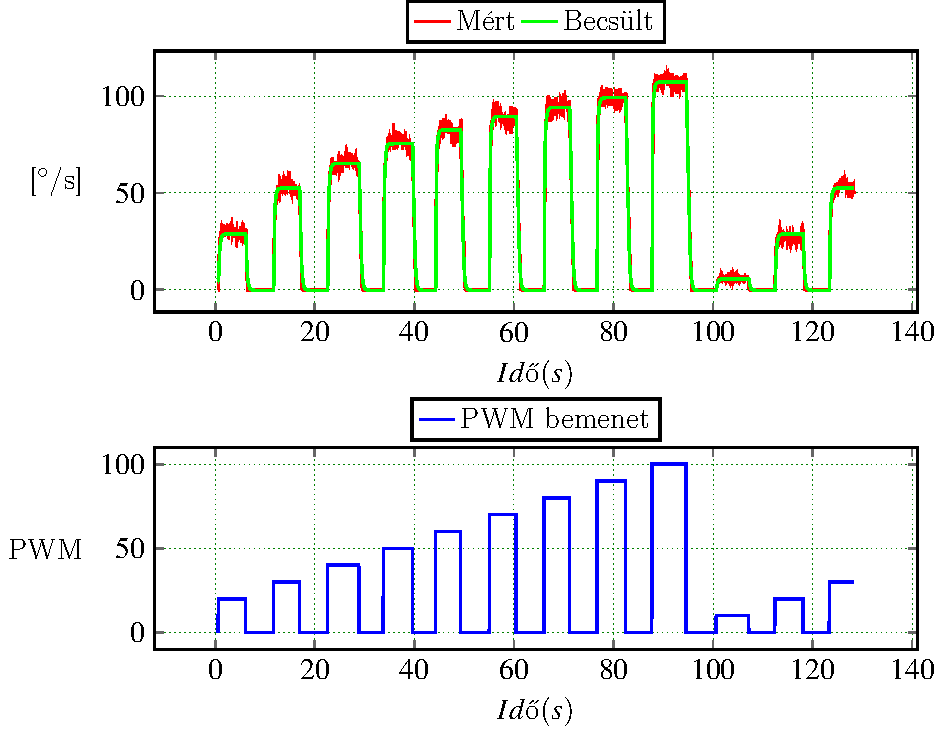
\includegraphics{tikz/NFsysIdent.pdf}
  \caption{Nagy fokozat Hammerstein-Wiener becsült modell válasza és a mért értékek.}
  \label{fig:NFsysIdent}
\end{figure}


Az átviteli függvény a bemenet 50/\% körül linearizálva.

\begin{equation}
    H_s(z)=\frac{-0.07017z^{-2} -0.053z^{-1}}{-0.2117^{-3}+0.7321z^{-2} -1.393z^{-1} +1}
\end{equation}

A tervezett PID szabályozó paramétere Kp: 7.11 , Ti: 23.66 , Td: 0.43

\subsection{Kisebbik fokozatban}

A becsült modellt összehasonlítva a mért értékekkel a \ref{fig:KFsysIdent}, a modell nem lineáris becsült modell megfelel a mért értékeknek.


\begin{figure}[H]
  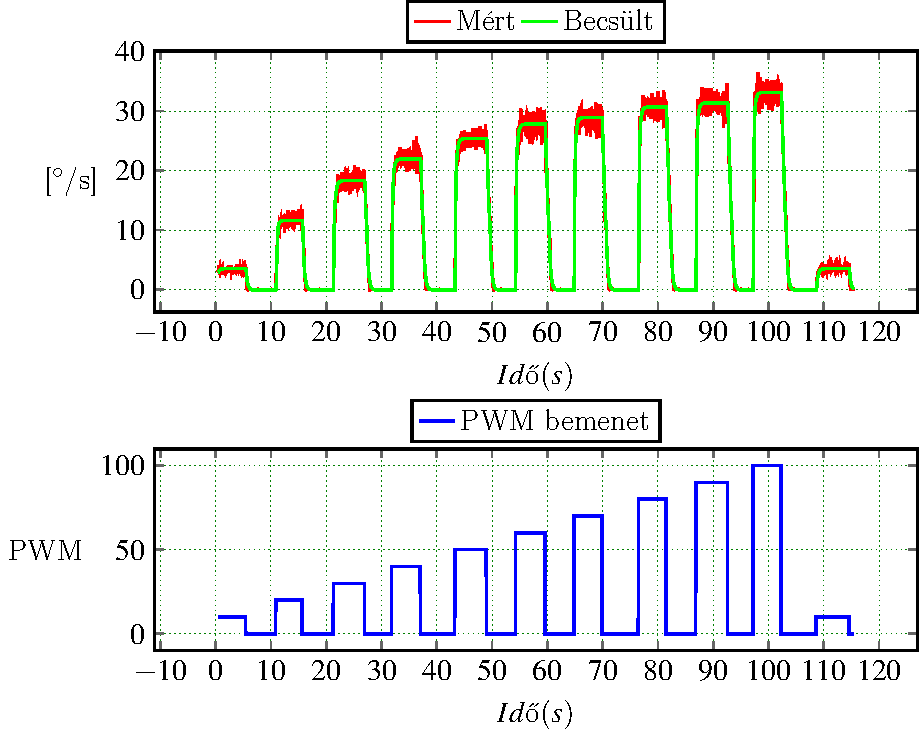
\includegraphics{tikz/KFsysIdent.pdf}
  \caption{Kis fokozat Hammerstein-Wiener becsült modell válasza és a mért értékek.}
  \label{fig:KFsysIdent}
\end{figure}

Az átviteli függvény a bemenet 50/\% körül linearizálva.

\begin{equation}
    H_s(z)=\frac{-0.0291z^{-2} -0.009263z^{-1}}{-0.198z^{-3}+0.7058z^{-2} -1.394z^{-1} +1}
\end{equation}

A tervezett PID szabályozó paraméterek: Kp: 15.96 , Ti:51.51 , Td:1.237 

.
